\section{Моделирование усилителя переменного тока в системе \textit{Multisim}}

\subsection{Усилитель с одной усилительной подсхемой на базе неинвернтирующего РУ}

Выполненная модель с согласно проведенным 
расчетам характеристиками элементов
представленна на рис.~\ref{fig:noninv_modeled}.

\begin{figure}[H]
	\centering
	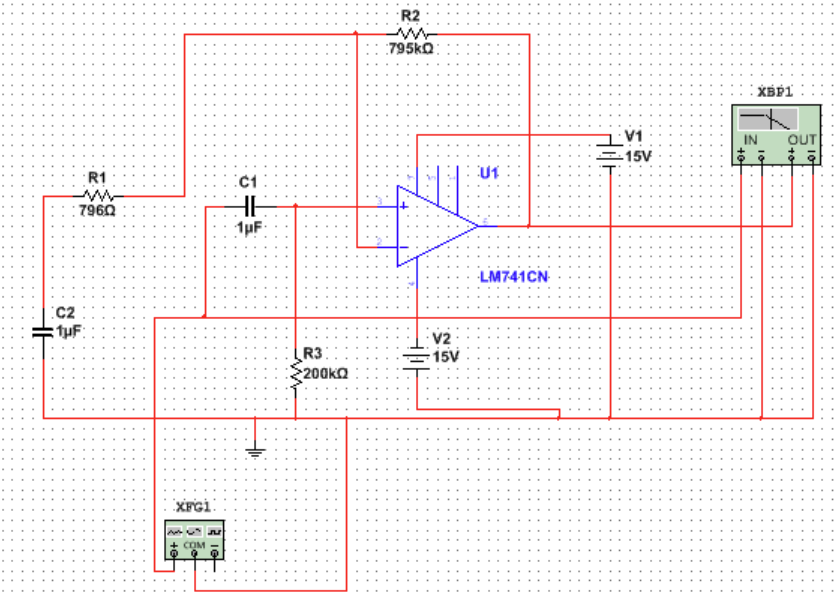
\includegraphics[width=0.7\linewidth]{photo/noninv_modeled}
	\caption{
		Схема (рис. \ref{fig:non_invertring_py}), 
		построенная в системе \textit{Multisim}. 
		Модель 
		усилителя переменного тока 
		с одной усилительной подсхемой
		на базе неинвернтирующего РУ
	}
	\label{fig:noninv_modeled}
\end{figure}

усилителя переменного тока
с двумя усилительными подсхемами
на базе инвертирующего и неинвертирующего РУ

\subsubsection*{Определение коэффициента усиления}

На рис.~\ref{fig:plot_k_noninv_py} показано 
определение коэффициента усиления
усилителя в полосе пропускания
по ЛАЧХ модели
усилителя переменного тока
с одной усилительной подсхемой
на базе неинвернтирующего РУ.
Его значение составляет:

$$ К_U = 997.47 $$

\begin{figure}[H]
	\centering
	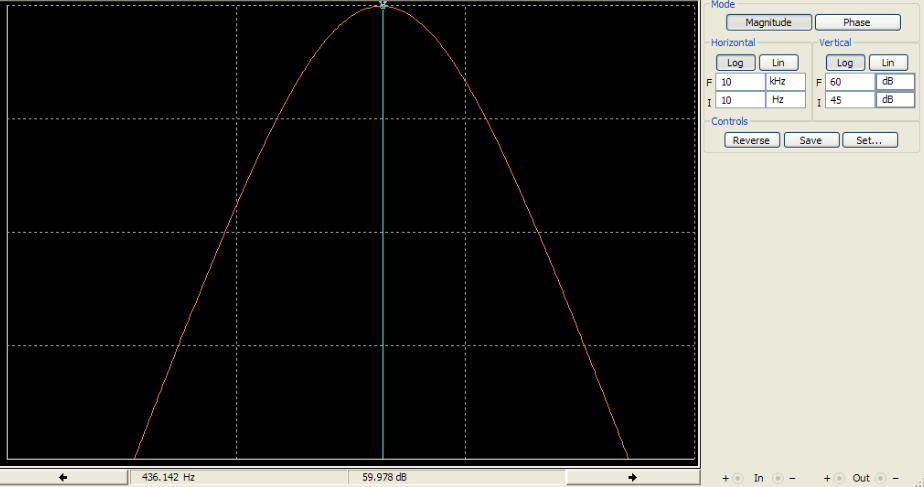
\includegraphics[width=0.7\linewidth]{photo/plot_k_noninv_py}
	\caption{Определение коэффициента усиления в дБ по ЛАЧХ модели}
	\label{fig:plot_k_noninv_py}
\end{figure}

Измеренный в cиcтеме \textit{Multisim}
коэффициент усиления $ К_U = 997.47 $ 
не сильно отличается от указанного 
в техническом задании $ K_U = 1000 $.

\subsubsection*{Определение верхней граничной частоты}

На рис.~\ref{fig:plot_f_high_noninv_py} показано 
определение верхней граничной частоты 
по ЛАЧХ модели
усилителя переменного тока
с одной усилительной подсхемой
на базе неинвернтирующего РУ.
Её значение составляет:

$$ f_в = 1.073~кГц $$.

\begin{figure}[H]
	\centering
	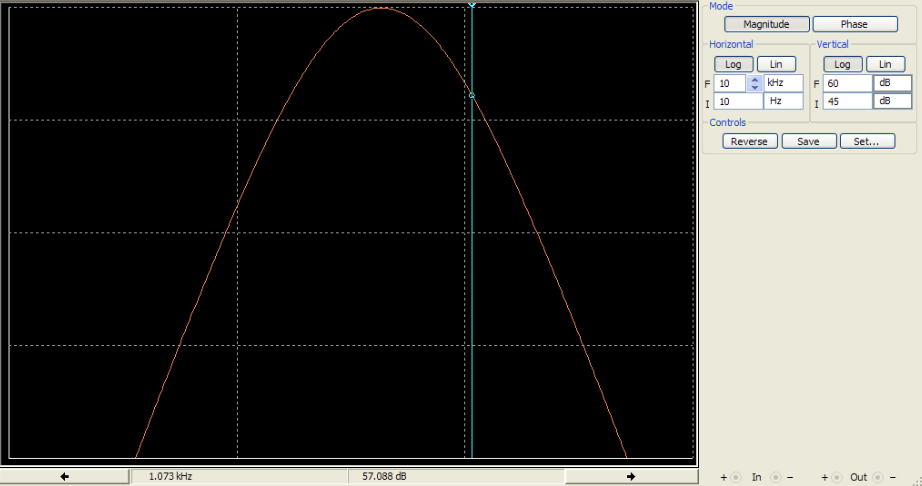
\includegraphics[width=0.7\linewidth]{photo/plot_f_high_noninv_py}
	\caption{Определение верхней граничной частоты по ЛАЧХ модели}
	\label{fig:plot_f_high_noninv_py}
\end{figure}

Для определения верхней граничной частоты 
определяем частоту для $ K_U - 3~дБ = 57~дБ $, 
сдвигая курсор вправо. 
Измеренное в системе \textit{Multisim} значение 
$ f_в = 1.073~кГц $ не удовлетворяет условию 
технического задания $ f_в \ge 20~кГц $.

\subsubsection*{Определение нижней граничной частоты}

На рис.~\ref{fig:plot_f_low_noninv_py} показано 
определение нижней граничной частоты
по ЛАЧХ модели
усилителя переменного тока
с одной усилительной подсхемой
на базе неинвернтирующего РУ.
Её значение составляет:

$$ f_н = 167.778~Гц $$

\begin{figure}[H]
	\centering
	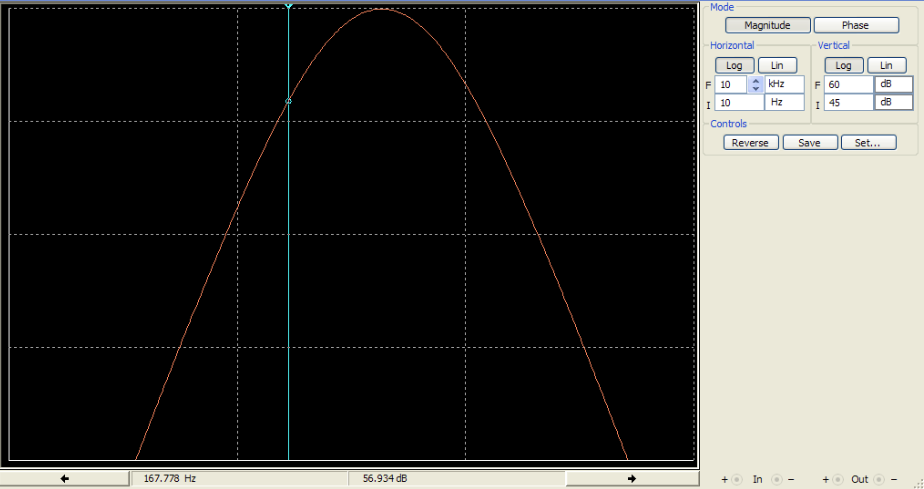
\includegraphics[width=0.7\linewidth]{photo/plot_f_low_noninv_py}
	\caption{Определение нижней граничной частоты по ЛАЧХ модели}
	\label{fig:plot_f_low_noninv_py}
\end{figure}

Для определения нижней граничной частоты 
определяем частоту для $ K_U - 3~дБ = 57~дБ $, 
сдвигая курсор влево. 
Измеренное в системе \textit{Multisim} значение 
$ f_н = 167.778~Гц $ не соответствует 
указанному в техническом задании $ f_н = 200~Гц $.

\subsubsection*{Вывод по анализу схемы}

Так как 
верхняя частота $ f_в~=~1.073~кГц $ и 
нижняя частота $ f_н~=~167.778~Гц $
для данной модели не соответствуют 
техническому заданию, в котором 
$ f_в \ge 20~кГц $ и
$ f_н = 200~Гц $
можно сделать вывод, что данная схема не подходит.

Усилитель имеет сравнительно низкую частоту $ f_в $ 
и небольшую полосу пропускания всего усилителя.

\subsection{Усилитель с двумя усилительными подсхемами}

Выполненная модель с согласно проведенным 
расчетам характеристиками элементов
представленна на рис.~\ref{fig:sub2_modeled}.

\begin{figure}[H]
	\centering
	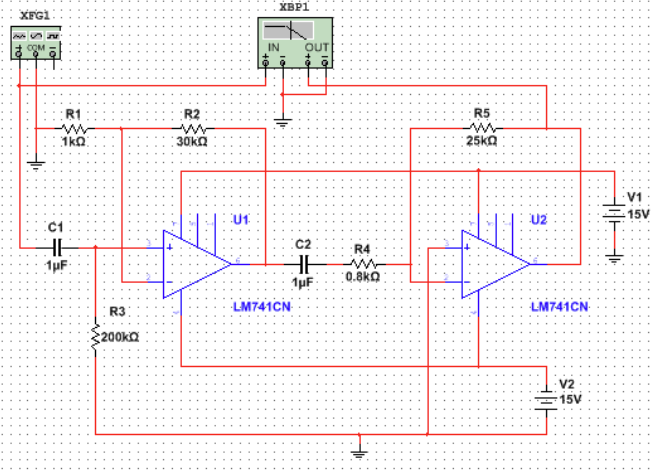
\includegraphics[width=0.7\linewidth]{photo/sub2_modeled}
	\caption{
		Схема (рис. \ref{fig:sub2_py}), 
		построенная в системе \textit{Multisim}. 
		Модель
		усилителя переменного тока
		с двумя усилительными подсхемами
		на базе инвертирующего и неинвертирующего РУ
	}
	\label{fig:sub2_modeled}
\end{figure}

\subsubsection*{Определение коэффициента усиления}

На рис.~\ref{fig:plot_k_sub2_py} показано 
определение коэффициента усиления 
усилителя в полосе пропускания 
по ЛАЧХ модели
усилителя переменного тока
с двумя усилительными подсхемами
на базе инвертирующего и неинвертирующего РУ. 
Его значение составляет:

$$ К_U = 997.47 $$.

\begin{figure}[H]
	\centering
	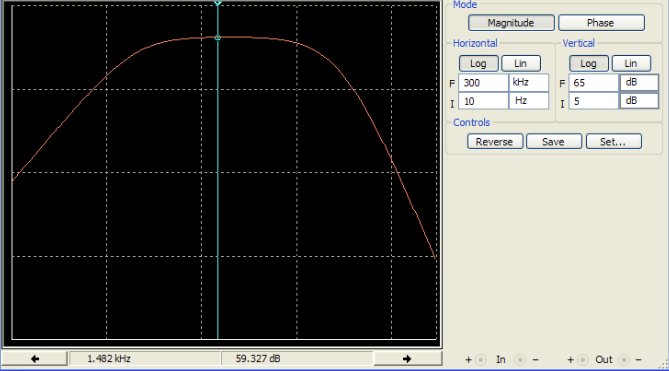
\includegraphics[width=0.7\linewidth]{photo/plot_k_sub2_py}
	\caption{Определение коэффициента усиления в дБ по ЛАЧХ модели}
	\label{fig:plot_k_sub2_py}
\end{figure}

Измеренный в cиcтеме \textit{Multisim}
коэффициент усиления $ К_U = 925.44 $ 
не сильно отличается от указанного 
в техническом задании $ K_U = 1000 $
с учётом погрешности.

\subsubsection*{Определение верхней граничной частоты}

На рис.~\ref{fig:plot_f_high_sub2_py} показано 
определение верхней граничной частоты 
по ЛАЧХ модели
усилителя переменного тока
с двумя усилительными подсхемами
на базе инвертирующего и неинвертирующего РУ. 
Её значение составляет:

$$ f_в = 21.083~кГц $$.

\begin{figure}[H]
	\centering
	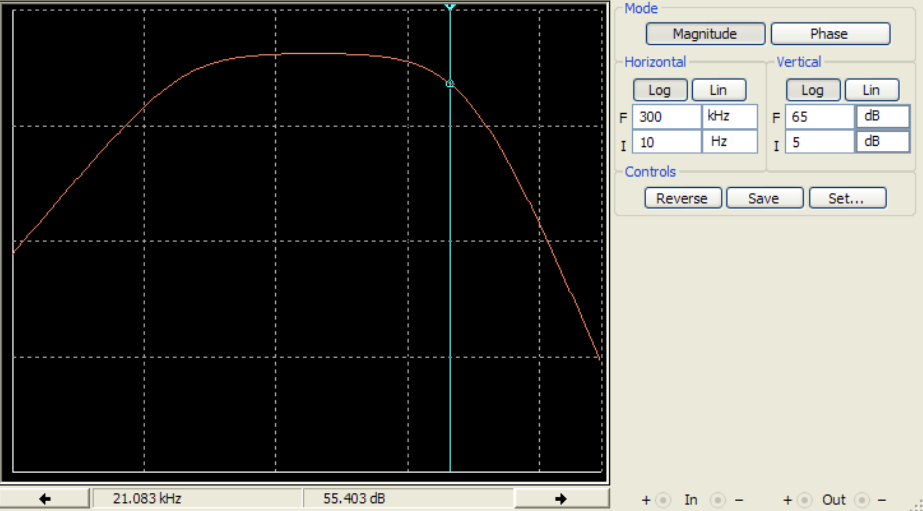
\includegraphics[width=0.7\linewidth]{photo/plot_f_high_sub2_py}
	\caption{Определение верхней граничной частоты по ЛАЧХ модели}
	\label{fig:plot_f_high_sub2_py}
\end{figure}

Для определения верхней граничной частоты 
определяем частоту для $ K_U - 3~дБ = 57~дБ $,
сдвигая курсор вправо. 
Измеренное в системе \textit{Multisim} значение 
$ f_в = 21.083~кГц $ удовлетворяет условию
технического задания $ f_в \ge 20~кГц $.

\subsubsection*{Определение нижней граничной частоты}

На рис.~\ref{fig:plot_f_low_sub2_py} показано 
определение нижней граничной частоты
по ЛАЧХ модели
усилителя переменного тока
с двумя усилительными подсхемами
на базе инвертирующего и неинвертирующего РУ. 
Её значение составляет:

$$ f_н = 232.485~Гц $$

\begin{figure}[H]
	\centering
	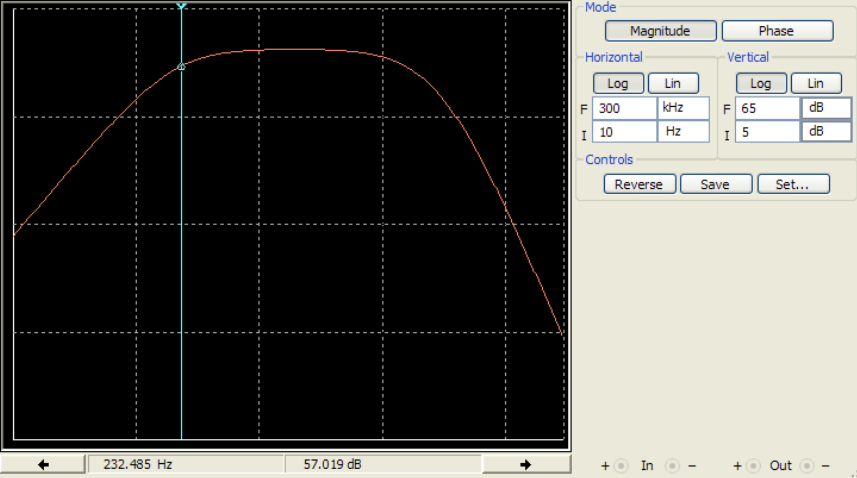
\includegraphics[width=0.7\linewidth]{photo/plot_f_low_sub2_py}
	\caption{Определение нижней граничной частоты по ЛАЧХ модели}
	\label{fig:plot_f_low_sub2_py}
\end{figure}

Для определения нижней граничной частоты 
определяем частоту для $ K_U - 3~дБ = 57~дБ $, 
сдвигая курсор влево. 
Измеренное в системе \textit{Multisim} значение 
$ f_н = 232.485~Гц $ соответствует 
указанному в техническом задании $ f_н = 200~Гц $
с учётом погрешности.

\subsubsection*{Вывод по анализу схемы}

Так как 
верхняя частота $ f_в = 21.083~кГц $
для данной модели соответствует техническому заданию,
в котором $ f_в \ge 20~кГц $ (c учётом погрешности) и
нижняя частота $ f_н = 232.485~Гц $
для данной модели соответствует техническому заданию,
в котором $ f_н = 200~Гц $ (с учётом погрешности),
можно сделать вывод, 
что схема на рис.~\ref{fig:sub2_py} подходит.

Данный усилитель имеет высокую частоту $ f_в $ и 
большую полосу пропускания всего усилителя.
